\documentclass{standalone}

\usepackage{siunitx}
\usepackage{pgfplots}
\usepackage{pgfplotstable}
\usepackage[utf8]{inputenc}

\begin{document}

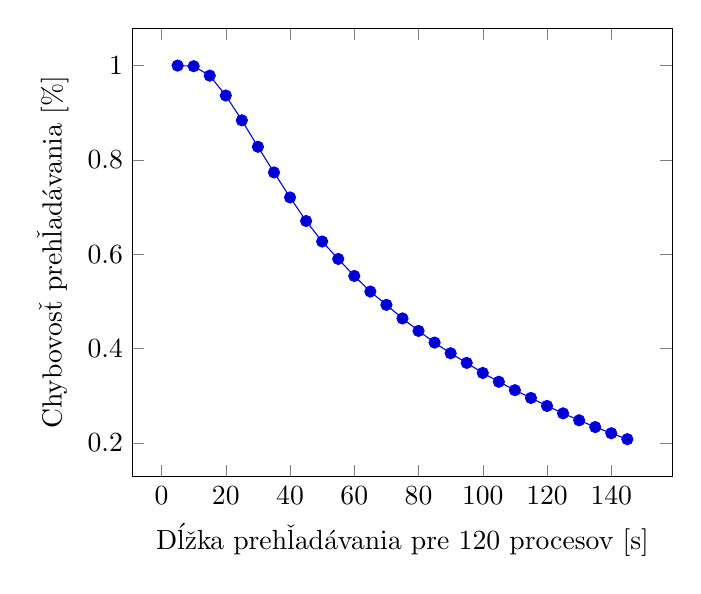
\begin{tikzpicture}
	\begin{axis}[
		xlabel={Dĺžka prehľadávania pre 120 procesov [s]},
		ylabel={Chybovosť prehľadávania [\%]}
	]

	\addplot coordinates{	
( 5, 1.00000000000000000000 )
( 10, .99869565217391304347 )
( 15, .97869565217391304347 )
( 20, .93652173913043478260 )
( 25, .88391304347826086956 )
( 30, .82782608695652173913 )
( 35, .77347826086956521739 )
( 40, .72043478260869565217 )
( 45, .67043478260869565217 )
( 50, .62695652173913043478 )
( 55, .59000000000000000000 )
( 60, .55391304347826086956 )
( 65, .52086956521739130434 )
( 70, .49260869565217391304 )
( 75, .46391304347826086956 )
( 80, .43739130434782608695 )
( 85, .41260869565217391304 )
( 90, .39000000000000000000 )
( 95, .36956521739130434782 )
( 100, .34826086956521739130 )
( 105, .32956521739130434782 )
( 110, .31173913043478260869 )
( 115, .29521739130434782608 )
( 120, .27826086956521739130 )
( 125, .26260869565217391304 )
( 130, .24782608695652173913 )
( 135, .23347826086956521739 )
( 140, .22043478260869565217 )
( 145, .20782608695652173913 )
    };
    \end{axis}
\end{tikzpicture}
    
\end{document}
